\section{Introduction}
% 介绍区块链交易系统背景
% Since the debut of Bitcoin in 2009 \cite{nakamoto2008bitcoin}, various cryptocurrencies and blockchain technology which provide decentralized environments for cryptocurrency transactions have gained increasing popularity and attention in recent years~\cite{wu2021analysis}. 
% Incorporating peer-to-peer (P2P) technology, cryptography, and consensus protocol, blochchain is regarded as the fundamental technology supporting cryptocurrencies and allows users to participate in cryptocurrency trading with pseudonyms~\cite{zhao2021temporal}.
The rapid development of blockchain technology has aroused great attention of businesses and researchers recently. By incorporating peer-to-peer networks, cryptography, and consensus protocols, blockchain \cite{zheng2018blockchain} achieves a decentralized environment for trading and brings new vitality to traditional industries. Particularly, the typical account-based blockchain platform Ethereum has opened the era of blockchain 2.0 through the introduction of smart contracts, giving blockchain various possibilities of application. However, the pseudonymous nature of blockchain has also attracted a variety of illegal transaction activities like financial scams and hacks.
% For example, a vulnerability of ``The DAO'' smart contract in Ethereum \cite{wood2014ethereum} was exploited by hackers in 2016, and a large amount of investment worth over \$70 million was stolen \cite{chainanalysis2016}.
% According to a report given by Chainalysis \cite{chainanalysis2019}, a blockchain data analysis service provider, cryptocurrency transactions with a total amount of more than \$11.5 billion worth of cryptocurrency transactions were associated with illegal transaction activities. % 这个报告是2019的
According to a recent report of Chainalysis \cite{chainalysis2022crime}, a famous blockchain security company, the losses caused by illegal transaction activities in cryptocurrency-related businesses have exceeded \$14 billion during 2021. Along with the boom of DeFi, most of these illegal trading activities and malicious attacks are conducted in the account-based blockchain trading systems like Ethereum and Binance Smart Chain (BSC) \cite{binancesmartchain} since the boom of DeFi.
% Due to the enforcement of the know-your-customer (KYC) process in some blockchain exchanges, illegal profits on many blockchain trading systems are usually laundered into concealed and ``clean'' fund flows before being cashed out. 
% Therefore, in order to crack down on illegal transaction activities on blockchain, a wealth of efforts from both academia and industry have been devoted to tracking the flow of funds involved in illegal transaction activities \cite{yousaf2019tracing,wulei2021www,di2015bitconeview}, the purpose being to understand real-world entities behind each transaction, help victims recover the losses, and thus make it easier to counter money laundering, fraud, dark web trading, and other digital asset crimes. 

%% 第二段  描述图1异常交易检测和交易追踪的区别
With the publicly accessible blockchain transaction data, various technologies have been developed to combat financial crimes in blockchain trading systems \cite{wu2021analysis}, and these technologies can be divided into two categories, namely \textbf{proactive (pre-trade) risk warning} and \textbf{remedial (post-trade) money tracking}. Proactive risk warning refers to evaluating the risk of new transactions according to the historical behaviors of the related accounts and the existing label information. Data-based fraud detection \cite{WhoAreThePhisher}, attack detection \cite{wu2021defiranger}, and other types of illegal transaction detection technologies \cite{weber2019anti} can be categorized in this scope. However, as shown in Figure \ref{fig:traditional_fraud_detection}, although proactive early warning can raise warnings for risky transactions before the occurrence of the trade, it cannot prevent the criminals who has already gotten the money from laundering and cashing out of the ill-gotten gains from exchanges since the pseudonymous and distributed nature of blockchain systems. Therefore, a wealth of efforts have been devoted to the remedial money tracking of the ill-gotten gains \cite{yousaf2019tracing,wulei2021www,di2015bitconeview}, aiming to deanonymize the related money flows and help victims recover the losses. 

Figure \ref{fig:blockchain_transaction_tracking} shows a toy example of the remedial money tracing. 
Generally speaking, transaction tracing starts from a source and traces the flow of money to the targets. Here, the source represents a tracing object such as the blockchain account of a fraudster decamping with a large number of ill-gotten gains, and the targets indicate the accounts used to gather the ``clean'' funds awaiting cashing out.
% Usually, the targets are addresses possessing the laundered funds or exchange deposit addresses. 
Though the identity information of accounts is unknown in blockchain systems, once we locate target deposit addresses of exchanges that enforce Know-Your-Customer (KYC) processes, the related criminals can be identified and caught off-chain according to the KYC information provided by the exchanges \cite{9332279}.
\begin{figure}[t]
    \centering
    \subfigure[Proactive risk warning in blockchain]{
        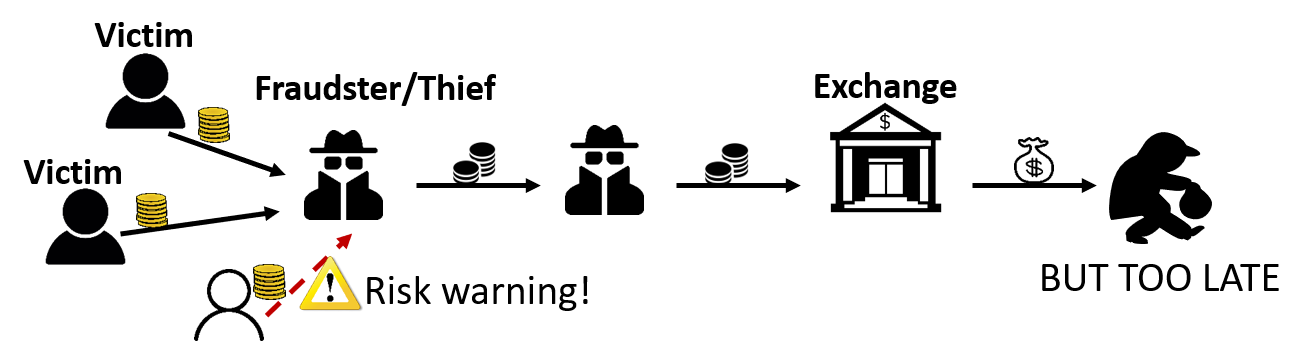
\includegraphics[width=0.8\linewidth]{figures/traditional_fraud_detection.png}
        \label{fig:traditional_fraud_detection}
    }
    
    \subfigure[Remedial money tracking in blockchain]{
        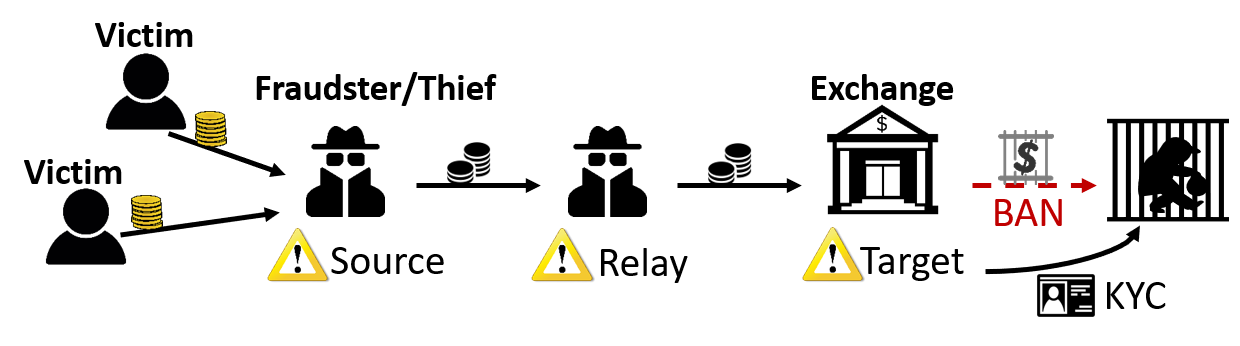
\includegraphics[width=0.8\linewidth]{figures/blockchain_transaction_tracking.png}
        \label{fig:blockchain_transaction_tracking}
    }
    \vspace{-0.1in}
    \caption{(a) Proactive risk warning in blockchain raises warnings for risky transactions. %However, it is always too late to prevent criminals from laundering and cashing out of the ill-gotten gains from exchanges. 
    (b) Remedial money tracking in blockchain traces the money flow among the source and the targets possessing the laundered funds, also providing evidence to catch the criminals off-chain.}
    % 不足以阻止已发生的损失
    \vspace{-0.1in}

\end{figure}

% 区块链交易系统上开展交易追踪的挑战
% Yet transaction tracking on blockchain trading systems is a rather challenging task.
% \textbf{\textit{Firstly}}, because of the pseudonymous nature of blockchain, it is unlikely to enforce the KYC process to verify the identities and ascertain the potential risks of users during cryptocurrency transactions \cite{wu2021analysis}, which makes it extremely difficult to determine the flow direction of a certain amount of money.
% \textbf{\textit{Secondly}}, without identity information, conducting money tracking in a large amount of blockchain transaction records is like finding a needle in the haystack, which requires a low computational cost of the transaction tracking.

% 当前工作的问题
% Current approaches for blockchain transaction tracking \cite{zhao2015graph,phetsouvanh2018egret,oggier2020ego} are mainly based on the Bitcoin system and inspired by graph searching \cite{xu2004fighting,abiteboul2003adaptive} and taint analysis \cite{moser2014towards,tironsakkul2019probing} technologies.
% The main idea of existing studies is to start from the source node and search the possible paths of funds between the source and target nodes via certain rules.
Current approaches for blockchain transaction tracing \cite{zhao2015graph,phetsouvanh2018egret,oggier2020ego,tironsakkul2019probing} are mainly based on rule-based heuristics and taint analysis~\cite{moser2014towards}. 
However, as an emerging research topic, existing transaction tracing methods have limitations in terms of universality, effectiveness and efficiency. Particularly, most existing heuristic methods are designed for specific scenarios based on experts experience, and cannot be automatically and intelligently applied to various blockchain transaction scenarios. In addition, the time cost and end conditions of existing methods, especially those requiring manual verification and intervention, is not definite or well defined, making their time efficiency and effectiveness difficult to guarantee.
% 然而,大多数现有方法通常依赖于专家经验来针对具体案例进行设计,因此很难自动且智能地适用于各类区块链交易场景(普适性)。此外,现有方法的时间复杂性较高,且没有确定的和well designed end condition,使用它们在巨大的交易网络中时犹如大海捞针一样时间效率和有效性都难以保障。
% However, as a newly emerging area, there still exist some limitations in much of the existing work:
% \textbf{(1)} Without theoretical proofs, the end condition of most of the existing methods relies on experts, which makes it difficult to estimate the computational cost of these methods.
% Therefore, the time cost of running existing transaction tracking methods on a large-scale transaction network may be extremely high when the end condition is not well designed.
% \textbf{(2)} Most of the existing studies are heuristic methods designed for some specific cases, which rely heavily on expert experience. Currently, there is no common framework and evaluation criteria for transaction tracking on blockchain. Therefore, it is difficult to evaluate the universality and superiority of the existing methods.
%However, most of the existing methods are designed for Bitcoin and some specific scenarios like cross-chain transactions \cite{yousaf2019tracing} and mixing transactions \cite{beres2020blockchain,wulei2021www}. 
%And they are inapplicable to deal with the transaction tracing task in account-based blockchain trading systems due to the different transaction models and the dependence on expert experience. 
%Moreover, due to the massive transaction data in account-based blockchains, tracing with the manual analysis method like finding a needle in the haystack. And it is difficult to quickly respond to security incidents. 
Besides, the popularity of DeFi in account-based blockchains like Ethereum and BSC brings many new kinds of semantics to blockchain transaction actions, leading to high barriers to the transaction tracing task.
% Yet transaction tracing in blockchain trading systems is a rather challenging task like finding a needle in the haystack due to the large amount of transaction data.

\begin{figure*}[t]
    \centering
    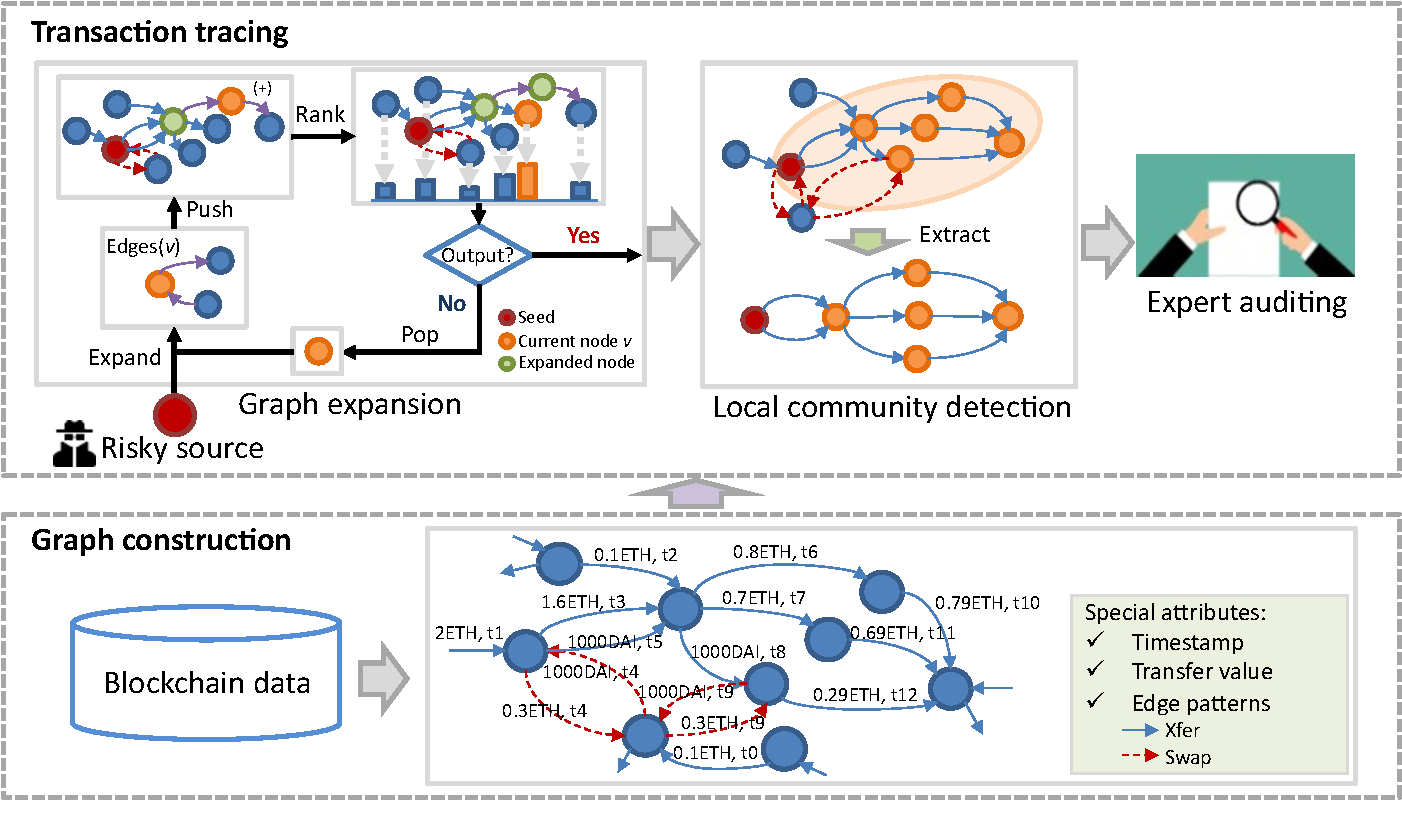
\includegraphics[width=0.65\linewidth]{figures/framework.pdf}
    \caption{The framework of TRacer.}
    \label{fig:TRacer}
\end{figure*}

% 介绍本文的思路
In this paper, we propose the first general tool called \textbf{\underline{T}\underline{R}acer}, which is a transaction \underline{T}racing in account-based blockchain trading systems incorporating Personalized Page\underline{R}ank-based technologies. Referring to the framework displayed in Figure \ref{fig:TRacer}, TRacer first models the blockchain transaction data including the complex DeFi operation actions into a directed, weighted, temporal, and multi-relationship graph, and then conducts local community detection on a subgraph around the risky seed obtained by graph expansion. The output small-scale community is the traced money flow graph and can be further audited by experts.
% Given a source, TRacer can automatically trace the money flow of the source.
% In order to solve the problems above, we propose a general transaction tracking framework on Blockchain trading systems named Push-Pop model, which tracks the fund flow about the source node.
% Then, we design the \textbf{Transaction Tracking Rank} (TTR) algorithm for the Push-Pop model based on personalized PageRank methods, where personalized PageRank is usually used to calculate node importance in a network from a point of view of a given node \cite{page1999pagerank}, ensuring the fund flow paths of the source node and the important nodes in the paths can be found.
% For the challenge brought by the pseudonymous nature, we utilize heuristic knowledge to design the TTR algorithm, so that the target nodes can obtain greater importance for identifying easier.
% we give the definition of transaction tracking on Blockchain trading systems as finding a local tracking network from the source node in which the paths among the source node and the nodes related to the source node can be found, and propose a general transaction tracking framework on Blockchain trading systems named Push-Pop model, which finds a local tracking network from the source node by a specific transaction tracking strategy.
% The transaction tracking strategy decides which nodes can be included in the local tracking network and we design the Transaction Tracking Rank (TTR) algorithm as the transaction tracking strategy of Push-Pop model, which chooses the important nodes of the source node constructing the local tracking network to ensure that the target nodes are more likely to be found in the local tracking network.
% 介绍本文对具体挑战和问题的解决方案
% For the challenge of the pseudonymous nature of Blockchain trading systems, we define the auditability of the local tracking network, which shows that the target nodes can be tracked if they are located in the local tracking network with labels or given in advance.
% 
Moreover, we propose a novel ranking algorithm based on personalized PageRank \cite{page1999pagerank} to reveal the relevance between the source and other accounts in blockchain systems. We introduce approximate personalized PageRank (APPR) \cite{andersen2006local,andersen2007local,yin2017local} to obtain the approximate solution of personalized PageRank, which can improve the scalability of the algorithm. Both graph expansion and local community detection in TRacer are based on the proposed ranking algorithm. 
%For the problems of effectiveness quantification, we design some metrics for understanding what kind of transaction tracking methods are effective. 
% It is worth mentioning that our proposed method has been applied and evaluated in transaction tracking tasks on several blockchain trading systems including Bitcoin, Ethereum, and Binance Smart Chain \cite{binancesmartchain} and so on, but may not be suitable for some privacy-enhancing blockchain trading systems like the Monero \cite{noether2014monero}. % 这些匿名系统都是UTXO上的
% Finally, we evaluate our method with metrics and network visualization analysis on five Ethereum transaction tracing cases.
Experimental results demonstrate the performance of TRacer on transaction tracing in account-based blockchains. The main contributions of this work can be summarized as follows:
\begin{itemize}
    % \item \textbf{Problem}: We give a problem definition of transaction tracking on Blockchain trading systems as finding the paths among the source node and the target nodes, and propose a general transaction tracking model named Push-Pop model.
    \item To the best of our knowledge, we are the first to study intelligent transaction tracing in account-based blockchain trading systems like Ethereum, which is an urgent problem with the booming security incidents in these systems.
    % \item \textbf{Approach}: We propose the TTR algorithm running on a transaction network, whose cost for convergence is $O(\frac{1}{\epsilon \alpha})$ controlled by two constant parameters of $\epsilon$ and $\alpha$. Additionally, we give the theoretical proof on how to set the parameters for ensuring our method is able to track the paths among the source node and the target nodes, even in the face of the worst conditions.
    \item We design and implement a general blockchain transaction tracing tool named TRacer, which is able to incorporate the complex semantics of transaction actions in DeFi. Particularly, a novel personalized PageRank method is employed to estimate the relevance score of accounts in TRacer.
    % \item \textbf{Evaluation}: We introduce metrics to quantify the effectiveness of transaction tracking methods on Blockchain trading systems, and experimental results demonstrate the priority of the proposed method. Moreover, we collect five standard datasets in Ethereum from real cases for blockchain transaction tracking and anti-money laundering research, and these codes for experiments were published on our Github\footnote{https://github.com/wuzhy1ng/BlockchainSpider}.
    % We thoroughly evaluate the proposed approach by comparing with the existing benchmarks on the historical loan data and achieved state-of-the-art performance. In addition, we conduct empirical studies in real-world risk control applications, and the result proves our method could prevent major financial losses for the financial institution
    \item We thoroughly evaluate the performance of TRacer via both theoretical analysis and experimental evaluation, and the results demonstrate the effectiveness and the scalability of TRacer. We also contribute a benchmark dataset verified by several security companies for evaluating the transaction tracing methods.
\end{itemize}

% 文章安排
% The rest of this paper is organized as follows. 
% Section \ref{sec:preliminaries} provides the preliminaries about this paper.
% A general transaction tracking framework Push-Pop model and the Transaction Tracking Rank algorithm are introduced in Section \ref{sec:proposed_approach}. 
% Evaluation and results are presented and discussed in Section \ref{sec:experiments}. 
% In Section \ref{sec:conclusion}, we conclude the paper and suggest directions for future work.
% Citations and appendices are at the end of this paper.
% \begin{figure}[htb]
%     \centering
%     \subfigure[A non-auditable transaction network]{
%         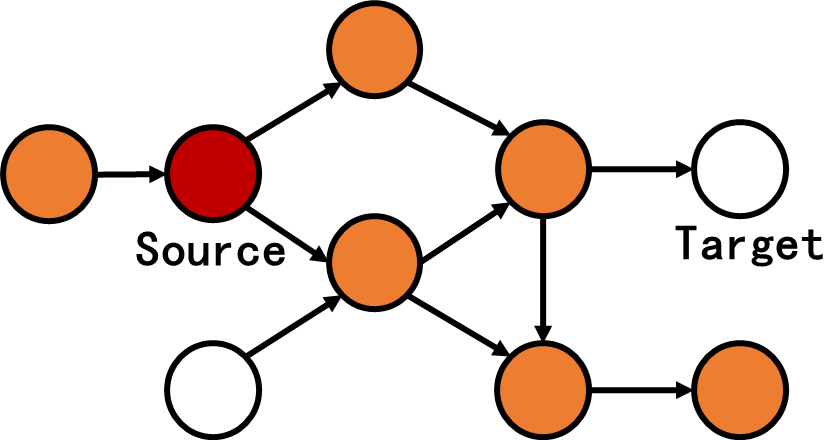
\includegraphics[width=0.46\linewidth,height=2cm]{figures/useless_tracking.png}
%         \label{fig:useless_tracking}
%     }
%     \subfigure[An auditable transaction network]{
%         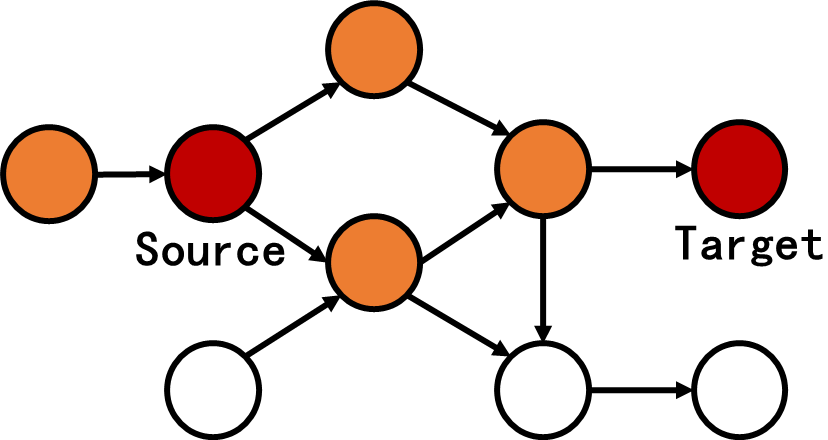
\includegraphics[width=0.46\linewidth,height=2cm]{figures/useful_tracking.png}
%         \label{fig:useful_tracking}
%     }
%     \caption{\color{red} Transaction networks with a source node as the center, where the local tracking network is colored.}
% \end{figure}

% In order to solve the cost problems, we propose heuristic knowledge to improve the local push procedure of the personalized PageRank (PPR) algorithms \cite{haveliwala2003topic,andersen2006local,andersen2007local,yin2017local,zhang2016approximate} for transaction tracking to achieve low-cost transaction tracking with theoretical proof, where PPR methods make a great difference in fraud detection \cite{van2017gotcha, ma2018graphrad} and graph neural networks \cite{klicpera2018predict,bojchevski2020scaling}.
% For the problems of how to quantify the effectiveness, we design some metrics for understanding what kind of transaction tracking methods is effective.

% 本文贡献
% Integrating the ideas above, we propose a general transaction tracking model named Push-Pop model, design the Transaction Tracking Rank (TTR) algorithm for calculating the personalized PageRank with heuristic knowledge proposed, and construct a TTR-based Push-Pop model for effective transaction tracking.


% ------------------我是一条分割线------------------------
% v1.0
% 介绍区块链
% For the past few years, Blockchain systems such as Bitcoin \cite{nakamoto2008bitcoin} have been gaining increasing popularity and attention, which provides a decentralized environment for transactions of cryptocurrencies.
% As the fundamental technology of cryptocurrency, Blockchain combines peer-to-peer (P2P) technology, cryptography, and consensus protocol, and allows the users to participate in transactions with pseudonymous accounts.
% With decentralized, traceable, immutable, and transparent nature, Blockchain is expected to be critical in the ``trust economy" of the future \cite{zhao2021temporal}.

% 介绍区块链上的犯罪现象
% However, the pseudonymous nature of Blockchain also attracts many illicit transaction activities like scams, extortion, money laundering, and so on.
% According to the statistics of Peckshield \cite{peckshield2021aml}, in the first half of 2021 alone, the losses caused by illegal transaction activities in cryptocurrency industry have exceeded \$14.24 billion. 
% % At the same time, cryptocurrency has gradually become a financing channel for terrorist organizations.
% Different from the traditional financial system, it is unlikely to enforce Know-Your-Customer (KYC) processes to verify the identities and ascertain the potential risks of users before conducting a cryptocurrency transaction \cite{wu2021analysis}, which makes it extremely difficult to audit the transactions on Blockchain.

% 监管者的解困之法-交易追踪
% On the other hand, the openness of transaction records on Blockchain also made a great difference in countering the illegal transaction activities on the Blockchain.
% Recent years have witnessed that researchers build transaction records on Blockchain as a transaction network and track the fund involved in illegal activities through transaction tracking technology to help victims recover their fund.

% 现有技术的总结和问题
% Current approaches \cite{zhao2015graph,phetsouvanh2018egret,xu2004fighting,oggier2020ego} for transaction tracking on Blockchain are mainly inspired by the graph searching \cite{xu2004fighting,abiteboul2003adaptive} and taint analysis \cite{moser2014towards,tironsakkul2019probing} technologies.
% And the main idea is to start from the source node and search the possible paths of fund among the source node and the target nodes through certain rules.
% Although the existing approaches are able to track the fund flow of some cases, there are still some key problems to be solved.
% \textit{Firstly}, without theoretical proofs, the end condition of most of the existing methods relies on experts, which makes it difficult to estimate the cost of methods.
% Therefore, existing transaction tracking methods search the transaction network on a large-scale with an extremely high cost if the end condition without well designed.
% \textit{Secondly}, the current researches have not given a standard about what kind of transaction tracking methods is powerful.
% In fact, the majority of methods verify their effectiveness in specific cases without considering the definition of metrics for quantifying the effectiveness of transaction tracking methods.

% \begin{figure*}[htb]
%     \centering
%     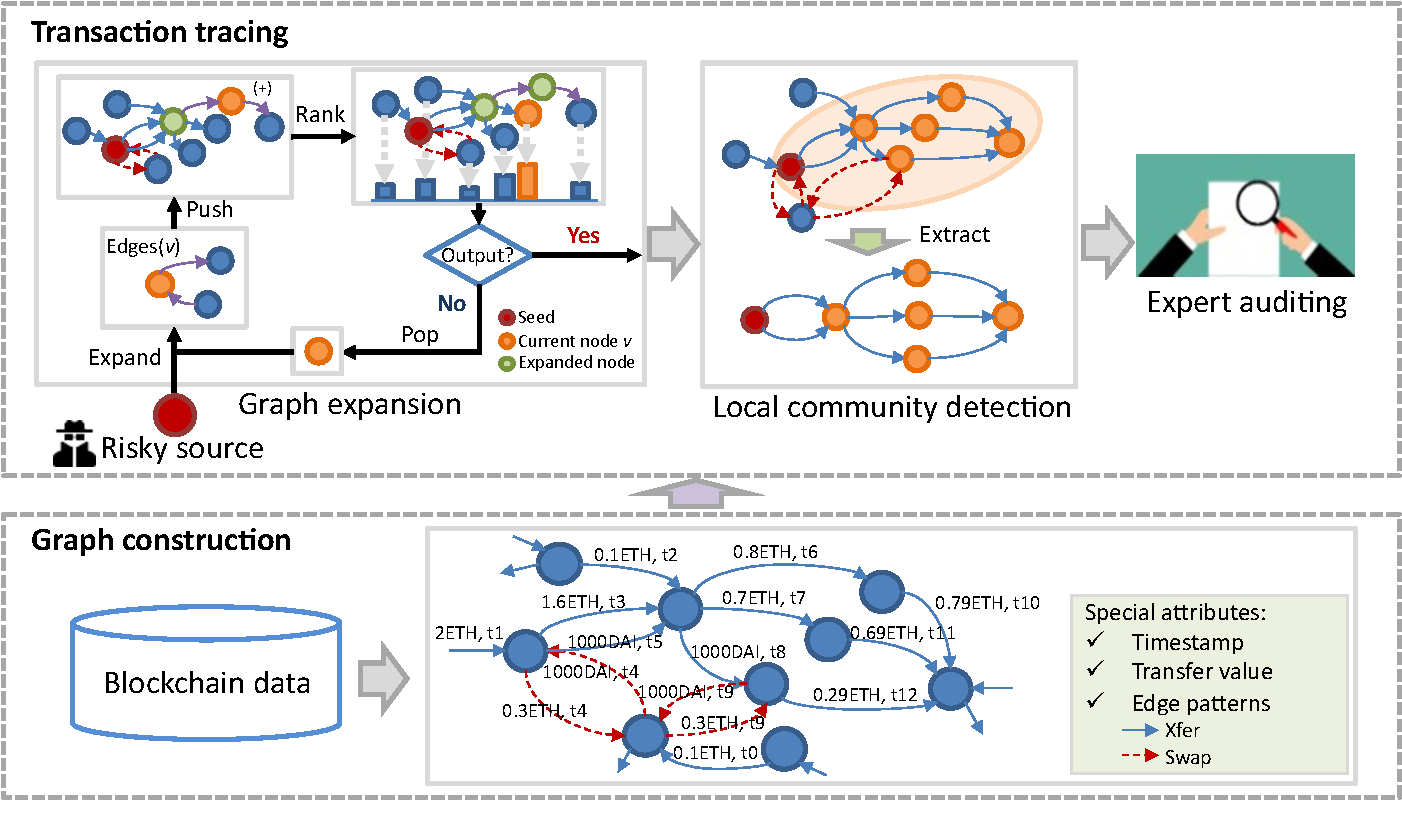
\includegraphics[width=\linewidth]{figures/framework.pdf}
%     \caption{Push-Pop Model, the general transaction tracking framework}
%     \label{fig:framework}
% \end{figure*}

% 顺带介绍一下APPR
% In order to solve the above problems, we have to introduce the personalized PageRank (PPR) \cite{haveliwala2003topic} that estimates the importance of other nodes to the source node in a given network.
% Vlasselaer et al. \cite{van2017gotcha} used PPR in social security fraud detection.
% Approximate Personalized PageRank (APPR) algorithms \cite{andersen2006local,andersen2007local,yin2017local,zhang2016approximate} can calculate the importance of the nodes in the local network to the source node with extremely low cost.
% Ma et al. \cite{ma2018graphrad} used APPR to find local fraud communities on large-scale networks.
% APPR also makes a difference in graph neural network.
% Compared with the original GCN, the performance of the APPR-based graph neural network gets an improvement significantly \cite{klicpera2018predict,bojchevski2020scaling}.

% 提出本文的方法
% Integrating the heuristic knowledge and the Approximate Personalized PageRank algorithm, we proposed our method named Transaction Tracking Rank (TTR), which evaluates the importance of each node for the source node in the transaction network of Blockchain.
% In addition, we give a general transaction tracking framework as the showing of Figure \ref{fig:framework} named as Push-Pop model.
% Our contribution could be listed as follow:
% \begin{itemize}
%     \item Based on the heuristic knowledge, we propose the TTR algorithm running on transaction network, whose cost for convergence within $O(\frac{1}{\epsilon \alpha})$ controlled by two constant parameters of $\epsilon$ and $\alpha$.
%     \item We design a general transaction tracking framework named as Push-Pop model for tracking the paths among the source node and the target nodes.
%     \item Using TTR as the strategy of the Push-Pop model, we give the upper bound of tracking depth starting from the source node and the condition of tracing from the source node to the target node in the worst case with theoretical proofs.
%     \item We give the metrics for understanding what kind of transaction tracking models is effective and the experiments with cases on Ethereum for verifying the effectiveness of our methods.
% \end{itemize}

% 行文思路
% The rest of this paper is organized as follows. 
% Section \ref{sec:preliminaries} gives the preliminaries about this paper.
% A general transaction tracking framework Push-Pop model and the Transaction Tracking Rank  are introduced in Section \ref{sec:proposed_approach}. 
% Evaluation and results are presented and discussed in Section \ref{sec:experiments}. 
% In Section \ref{sec:conclusion}, we conclude the paper and suggest directions for future work.
% Citations at the end of this paper.